% Informe del laboratorio 5: gemelo digital, discretización, propiedades estructurales y triggers de seguridad
% Compilar desde esta carpeta: pdflatex informe_lab05.tex (dos veces)
\documentclass[a4paper,11pt]{article}
% Preámbulo común de los informes de laboratorio (II/2026). Se incluye desde desarrollo/fuentes/laboratorios/labNN_*/
%   % Preámbulo común de los informes de laboratorio (II/2026). Se incluye desde desarrollo/fuentes/laboratorios/labNN_*/
%   % Preámbulo común de los informes de laboratorio (II/2026). Se incluye desde desarrollo/fuentes/laboratorios/labNN_*/
%   \input{../informe_comun}
\input{../../gemelo-digital/manual/estilo_manual}
\input{../../gemelo-digital/manual/tecnico/macros}
% Las rutas son relativas a la carpeta de cada informe (desarrollo/fuentes/laboratorios/labNN/): las fuentes
% (estilo, imágenes del manual, figuras y levantamiento) están en desarrollo/fuentes; los entregables públicos
% (planos, base de datos) cuatro niveles más arriba, en semestres/2026_II/.
\graphicspath{{../../../../documentacion/planos_isa/pid/}{../../../../documentacion/planos_isa/electrico/}{../../../../documentacion/manuales_inversa/}
  {../../../../database/mockups/}{../../../../database/documentacion/}{../../../../database/modelo/}{../../../../database/interfaz/}
  {../../gemelo-digital/manual/img/}{../../modelo-3d/informe/figuras/}{../../modelo-3d/levantamiento/}{../../../../../../global/fotos-planta/}}
\usepackage{pdflscape}
\lstset{showstringspaces=false}
% plano A3 en una página apaisada: \plano[página]{archivo}{leyenda}
\newcommand{\plano}[3][1]{\begin{landscape}\begin{figure}[p]\centering\includegraphics[page=#1, width=\linewidth, height=0.86\textwidth, keepaspectratio]{#2}\caption{#3}\end{figure}\end{landscape}}
\setlength{\headheight}{14pt}
\newcommand{\nlab}{}
\newcommand{\tlab}{}
% tipo de documento en la portada y el encabezado (los documentos de logros los redefinen)
\newcommand{\tipodoc}{Informe del Laboratorio Integrado}
\newcommand{\tipocab}{Informe del laboratorio}
\lhead{\small Brazo XK-JS1-1 · \tipocab{} \nlab}
\rhead{\small UMSA · II/2026}

% \portada{número}{título}{inicio}{entrega}{semanas}
\newcommand{\portada}[5]{%
\renewcommand{\nlab}{#1}%
\begin{titlepage}
\centering
\vspace*{0.6cm}
{\large Universidad Mayor de San Andrés · Facultad de Ingeniería\par}
{\large Carrera de Ingeniería Electrónica\par}
\vspace{0.8cm}
{\color{naranja!80!black}\rule{\linewidth}{1.5pt}\par}
\vspace{0.3cm}
{\Large \tipodoc{} Nº #1\par}
\vspace{0.2cm}
{\huge\bfseries #2\par}
\vspace{0.3cm}
{\color{naranja!80!black}\rule{\linewidth}{1.5pt}\par}
\vspace{0.8cm}
{\large Planta: brazo robótico XK-JS1-1 de 4 grados de libertad\par}
\vspace{0.3cm}
{\large ETN-902 Sistemas de Control II · ETN-1034 Aplicación de Técnicas de Control · ETN-1000 Bases de Datos\par}
\vspace{1cm}
\begin{tabular}{rl}
\textbf{Docente:} & Ing. Jorge Antonio Nava Amador\\
\textbf{Auxiliares:} & Limber Ajnota · Fabián Plata · Franz Choque\\
\textbf{Inicio de trabajo:} & #3\\
\textbf{Entrega:} & #4 (#5)\\
\end{tabular}
\vspace{1cm}

\begin{tabular}{ll}
\multicolumn{2}{l}{\textbf{Escuadra del brazo de 4 GDL}}\\[2pt]
Control (ETN-902 / ETN-1034): & Gabriel Andres Gomez Calla\\
 & Jose Lenin Mamani Choque\\
 & Miguel Alejandro Lima Huarachi\\
 & Román Abner Machicado Arequipa\\[2pt]
Cómputo (ETN-1000): & Miguel Alejandro Lima Huarachi\\
 & Marco Eduardo Chura Rondo\\
\end{tabular}
\vfill
{\small Repositorio: \url{https://github.com/GabAndGom/Brazo-de-4-grados-de-libertad}\par}
{\small La Paz, Bolivia · gestión II/2026\par}
\end{titlepage}
}

% Tabla de entregables (Definition of Done): \begin{dod} ... \end{dod}, filas: entregable & estado & evidencia\\
\newenvironment{dod}{\begin{center}\small\begin{longtable}{>{\raggedright}p{5.2cm} >{\raggedright}p{1.8cm} >{\raggedright\arraybackslash}p{7.6cm}}
\toprule \textbf{Entregable} & \textbf{Estado} & \textbf{Evidencia / observación}\\ \midrule \endhead}
{\bottomrule\end{longtable}\end{center}}

% Estilo común de los manuales del gemelo digital (se incluye con \input)
\usepackage{geometry}
\geometry{letterpaper, margin=2.2cm}
\usepackage[spanish, es-nodecimaldot, mexico]{babel}
\usepackage[utf8]{inputenc}
\usepackage[T1]{fontenc}
\usepackage{lmodern}
\usepackage{amsmath,amssymb}
\usepackage[table]{xcolor}
\definecolor{naranja}{RGB}{194,98,12}
\definecolor{rojo}{RGB}{192,57,43}
\definecolor{verde}{RGB}{30,120,70}
\definecolor{azulw}{RGB}{0,103,184}
\definecolor{azulg}{RGB}{70,90,120}
\definecolor{gris}{RGB}{242,242,242}
\definecolor{grisos}{RGB}{90,90,90}
\usepackage{booktabs,longtable,array,tabularx}
\usepackage{graphicx}
\usepackage{float}
\usepackage{caption}
\captionsetup{font=small, labelfont=bf}
\usepackage{tikz}
\usetikzlibrary{positioning,arrows.meta,fit,calc,shapes.geometric,decorations.pathreplacing,backgrounds}
\usepackage{enumitem}
\setlist{itemsep=2pt}
\usepackage{listings}
\lstset{basicstyle=\ttfamily\small, frame=single, backgroundcolor=\color{gris}, breaklines=true,
  columns=fullflexible, keepspaces=true, extendedchars=true, upquote=true,
  literate={á}{{\'a}}1 {é}{{\'e}}1 {í}{{\'i}}1 {ó}{{\'o}}1 {ú}{{\'u}}1 {ñ}{{\~n}}1 {Á}{{\'A}}1 {É}{{\'E}}1
           {Í}{{\'I}}1 {Ó}{{\'O}}1 {Ú}{{\'U}}1 {Ñ}{{\~N}}1 {ü}{{\"u}}1 {¿}{{?`}}1 {¡}{{!`}}1 {…}{{...}}3
           {θ}{{$\theta$}}1 {·}{{$\cdot$}}1 {«}{{\guillemotleft}}1 {»}{{\guillemotright}}1 {°}{{$^\circ$}}1}
\usepackage{hyperref}
\hypersetup{colorlinks=true, linkcolor=naranja, urlcolor=naranja}
\usepackage{fancyhdr}
\pagestyle{fancy}
\fancyhf{}
\cfoot{\small \thepage}
\newcommand{\codigo}[1]{\texttt{#1}}
\newcommand{\archivo}[1]{\textbf{\texttt{#1}}}
\newcommand{\aviso}[1]{\par\smallskip\noindent\colorbox{rojo!10}{\parbox{\dimexpr\linewidth-2\fboxsep}{\textbf{\color{rojo}Atención.} #1}}\par\smallskip}
\newcommand{\nota}[1]{\par\smallskip\noindent\colorbox{gris}{\parbox{\dimexpr\linewidth-2\fboxsep}{#1}}\par\smallskip}
\tikzset{
  marca/.style={circle, fill=naranja, text=white, font=\bfseries\footnotesize, inner sep=1.4pt, minimum size=4.6mm, draw=white, line width=0.8pt},
  caja/.style={draw, rounded corners=2pt, fill=gris, align=center, font=\small, minimum height=10mm, inner sep=4pt},
  cajab/.style={caja, fill=white},
  cajan/.style={caja, fill=naranja!14, draw=naranja!70!black},
  paso/.style={draw, rounded corners=2pt, fill=white, align=left, font=\small, text width=3.4cm, minimum height=15mm, inner sep=5pt},
  num/.style={circle, fill=naranja, text=white, font=\bfseries\small, inner sep=1.5pt, minimum size=6mm},
  flecha/.style={-{Stealth[length=2.2mm]}, thick},
  dflecha/.style={{Stealth[length=2.2mm]}-{Stealth[length=2.2mm]}, thick},
  etiq/.style={font=\scriptsize, align=center},
}
\DeclareRobustCommand{\num}[1]{\tikz[baseline=-0.7ex]\node[marca]{#1};}
% \captura{ancho}{archivo}{marcas en coordenadas 0-1 desde la esquina inferior izquierda}
\newcommand{\captura}[3]{%
  \begin{tikzpicture}
  \node[anchor=south west, inner sep=0, draw=black!25] (img) {\includegraphics[width=#1]{#2}};
  \begin{scope}[x={(img.south east)}, y={(img.north west)}]
  #3
  \end{scope}
  \end{tikzpicture}}
% ventana dibujada (consolas y diálogos): \ventana{ancho}{alto}{título}{contenido}
\newcommand{\ventana}[4]{%
\begin{tikzpicture}
\node[draw=black!50, fill=white, minimum width=#1, minimum height=#2, anchor=north west, inner sep=0] (v) at (0,0) {};
\fill[black!8] (v.north west) rectangle ($(v.north east)+(0,-6mm)$);
\node[anchor=west, font=\scriptsize] at ($(v.north west)+(2mm,-3mm)$) {#3};
\node[anchor=east, font=\scriptsize] at ($(v.north east)+(-2mm,-3mm)$) {--\quad$\square$\quad$\times$};
\node[anchor=north west, inner sep=3mm, text width=#1-6mm, font=\scriptsize\ttfamily, align=left] at ($(v.north west)+(0,-6mm)$) {#4};
\end{tikzpicture}}

% Macros del manual técnico: ladder, estados, código y rutas de imágenes
\usetikzlibrary{shapes.multipart}
\graphicspath{{../img/}{../../../../../../../global/fotos-planta/}{../../../modelo-3d/informe/figuras/}{../../../modelo-3d/levantamiento/}{../../../../../database/modelo/}{../../../../../documentacion/manuales_inversa/}{../../../../../documentacion/planos_isa/electrico/}{../../../../../database/interfaz/}}

\lstdefinestyle{py}{language=Python, keywordstyle=\color{azulg}\bfseries, commentstyle=\color{grisos}\itshape,
  stringstyle=\color{verde}, basicstyle=\ttfamily\scriptsize, numbers=left, numberstyle=\tiny\color{grisos}}
\lstdefinestyle{js}{language=Java, morekeywords={const,let,function,async,await,return,for,of,if,else}, keywordstyle=\color{azulg}\bfseries,
  commentstyle=\color{grisos}\itshape, stringstyle=\color{verde}, basicstyle=\ttfamily\scriptsize, numbers=left, numberstyle=\tiny\color{grisos}}
\lstdefinestyle{awl}{basicstyle=\ttfamily\tiny, commentstyle=\color{grisos}\itshape, morecomment=[l]{//},
  keywordstyle=\color{azulg}\bfseries, morekeywords={LD,LDN,A,AN,O,ON,EU,ED,S,R,MOVB,MOVW,MOVD,PLS,TON,CALL,CRET,LPS,LRD,LPP,ALD,OLD,FILL,LDW,LDB,LDD,AW,AD,AB,OW,OD},
  numbers=left, numberstyle=\tiny\color{grisos}, frame=single, backgroundcolor=\color{gris}}
\lstdefinestyle{sql}{language=SQL, keywordstyle=\color{azulg}\bfseries, commentstyle=\color{grisos}\itshape,
  stringstyle=\color{verde}, basicstyle=\ttfamily\tiny, numbers=left, numberstyle=\tiny\color{grisos},
  morekeywords={REFERENCES,SERIAL,SMALLSERIAL,BIGSERIAL,TIMESTAMPTZ,BOOLEAN,INET,RETURNS,TRIGGER,LANGUAGE,DECLARE,RAISE,EXCEPTION,VIEW,INDEX}}

\tikzset{
  ld/.style={line width=0.7pt},
  pics/na/.style={code={\fill[white](-0.12,-0.26) rectangle (0.12,0.26);
     \draw[thick](-0.1,-0.24)--(-0.1,0.24)(0.1,-0.24)--(0.1,0.24);
     \node[font=\scriptsize\ttfamily, above] at (0,0.22){#1};}},
  pics/nc/.style={code={\fill[white](-0.12,-0.26) rectangle (0.12,0.26);
     \draw[thick](-0.1,-0.24)--(-0.1,0.24)(0.1,-0.24)--(0.1,0.24);\draw(-0.17,-0.24)--(0.17,0.24);
     \node[font=\scriptsize\ttfamily, above] at (0,0.22){#1};}},
  pics/pf/.style={code={\fill[white](-0.12,-0.26) rectangle (0.12,0.26);
     \draw[thick](-0.1,-0.24)--(-0.1,0.24)(0.1,-0.24)--(0.1,0.24);
     \node[font=\tiny\bfseries] at (0,0){P};}},
  pics/cmp/.style n args={3}{code={\fill[white](-0.12,-0.26) rectangle (0.12,0.26);
     \draw[thick](-0.1,-0.24)--(-0.1,0.24)(0.1,-0.24)--(0.1,0.24);
     \node[font=\tiny\ttfamily] at (0,0){#2};
     \node[font=\scriptsize\ttfamily, above] at (0,0.22){#1};
     \node[font=\scriptsize\ttfamily, below] at (0,-0.22){#3};}},
  pics/bob/.style n args={3}{code={\fill[white](-0.2,-0.26) rectangle (0.2,0.26);
     \draw[thick](-0.05,0.24) arc (110:250:0.255);\draw[thick](0.05,0.24) arc (70:-70:0.255);
     \node[font=\tiny\bfseries] at (0,0){#2};
     \node[font=\scriptsize\ttfamily, above] at (0,0.22){#1};
     \node[font=\scriptsize\ttfamily, below] at (0,-0.22){#3};}},
  fb/.style={draw, fill=white, font=\scriptsize\ttfamily, align=left, inner sep=3pt, anchor=west},
  barra/.style={line width=2pt},
  estado/.style={draw, rounded corners=3pt, fill=white, align=center, font=\scriptsize, minimum width=22mm, minimum height=10mm, inner sep=3pt},
  estadon/.style={estado, fill=naranja!14, draw=naranja!70!black},
  trans/.style={font=\scriptsize, align=center, fill=white, inner sep=1pt},
  lugar/.style={circle, draw, thick, minimum size=7mm, fill=white},
  transicion/.style={rectangle, fill=black, minimum width=1.6mm, minimum height=7mm, inner sep=0},
  tabla/.style={rectangle split, rectangle split parts=2, draw, fill=white, font=\tiny\ttfamily, align=left, inner sep=2pt, rounded corners=1pt, text width=33mm},
}
\newcommand{\pendiente}[1]{\par\smallskip\noindent\colorbox{naranja!12}{\parbox{\dimexpr\linewidth-2\fboxsep}{\textbf{\color{naranja!80!black}Pendiente.} #1}}\par\smallskip}
\newcommand{\cumple}{\textcolor{verde}{\textbf{cumplido}}}
\newcommand{\parcial}{\textcolor{naranja}{\textbf{parcial}}}
\newcommand{\falta}{\textcolor{rojo}{\textbf{pendiente}}}

% Las rutas son relativas a la carpeta de cada informe (desarrollo/fuentes/laboratorios/labNN/): las fuentes
% (estilo, imágenes del manual, figuras y levantamiento) están en desarrollo/fuentes; los entregables públicos
% (planos, base de datos) cuatro niveles más arriba, en semestres/2026_II/.
\graphicspath{{../../../../documentacion/planos_isa/pid/}{../../../../documentacion/planos_isa/electrico/}{../../../../documentacion/manuales_inversa/}
  {../../../../database/mockups/}{../../../../database/documentacion/}{../../../../database/modelo/}{../../../../database/interfaz/}
  {../../gemelo-digital/manual/img/}{../../modelo-3d/informe/figuras/}{../../modelo-3d/levantamiento/}{../../../../../../global/fotos-planta/}}
\usepackage{pdflscape}
\lstset{showstringspaces=false}
% plano A3 en una página apaisada: \plano[página]{archivo}{leyenda}
\newcommand{\plano}[3][1]{\begin{landscape}\begin{figure}[p]\centering\includegraphics[page=#1, width=\linewidth, height=0.86\textwidth, keepaspectratio]{#2}\caption{#3}\end{figure}\end{landscape}}
\setlength{\headheight}{14pt}
\newcommand{\nlab}{}
\newcommand{\tlab}{}
% tipo de documento en la portada y el encabezado (los documentos de logros los redefinen)
\newcommand{\tipodoc}{Informe del Laboratorio Integrado}
\newcommand{\tipocab}{Informe del laboratorio}
\lhead{\small Brazo XK-JS1-1 · \tipocab{} \nlab}
\rhead{\small UMSA · II/2026}

% \portada{número}{título}{inicio}{entrega}{semanas}
\newcommand{\portada}[5]{%
\renewcommand{\nlab}{#1}%
\begin{titlepage}
\centering
\vspace*{0.6cm}
{\large Universidad Mayor de San Andrés · Facultad de Ingeniería\par}
{\large Carrera de Ingeniería Electrónica\par}
\vspace{0.8cm}
{\color{naranja!80!black}\rule{\linewidth}{1.5pt}\par}
\vspace{0.3cm}
{\Large \tipodoc{} Nº #1\par}
\vspace{0.2cm}
{\huge\bfseries #2\par}
\vspace{0.3cm}
{\color{naranja!80!black}\rule{\linewidth}{1.5pt}\par}
\vspace{0.8cm}
{\large Planta: brazo robótico XK-JS1-1 de 4 grados de libertad\par}
\vspace{0.3cm}
{\large ETN-902 Sistemas de Control II · ETN-1034 Aplicación de Técnicas de Control · ETN-1000 Bases de Datos\par}
\vspace{1cm}
\begin{tabular}{rl}
\textbf{Docente:} & Ing. Jorge Antonio Nava Amador\\
\textbf{Auxiliares:} & Limber Ajnota · Fabián Plata · Franz Choque\\
\textbf{Inicio de trabajo:} & #3\\
\textbf{Entrega:} & #4 (#5)\\
\end{tabular}
\vspace{1cm}

\begin{tabular}{ll}
\multicolumn{2}{l}{\textbf{Escuadra del brazo de 4 GDL}}\\[2pt]
Control (ETN-902 / ETN-1034): & Gabriel Andres Gomez Calla\\
 & Jose Lenin Mamani Choque\\
 & Miguel Alejandro Lima Huarachi\\
 & Román Abner Machicado Arequipa\\[2pt]
Cómputo (ETN-1000): & Miguel Alejandro Lima Huarachi\\
 & Marco Eduardo Chura Rondo\\
\end{tabular}
\vfill
{\small Repositorio: \url{https://github.com/GabAndGom/Brazo-de-4-grados-de-libertad}\par}
{\small La Paz, Bolivia · gestión II/2026\par}
\end{titlepage}
}

% Tabla de entregables (Definition of Done): \begin{dod} ... \end{dod}, filas: entregable & estado & evidencia\\
\newenvironment{dod}{\begin{center}\small\begin{longtable}{>{\raggedright}p{5.2cm} >{\raggedright}p{1.8cm} >{\raggedright\arraybackslash}p{7.6cm}}
\toprule \textbf{Entregable} & \textbf{Estado} & \textbf{Evidencia / observación}\\ \midrule \endhead}
{\bottomrule\end{longtable}\end{center}}

% Estilo común de los manuales del gemelo digital (se incluye con \input)
\usepackage{geometry}
\geometry{letterpaper, margin=2.2cm}
\usepackage[spanish, es-nodecimaldot, mexico]{babel}
\usepackage[utf8]{inputenc}
\usepackage[T1]{fontenc}
\usepackage{lmodern}
\usepackage{amsmath,amssymb}
\usepackage[table]{xcolor}
\definecolor{naranja}{RGB}{194,98,12}
\definecolor{rojo}{RGB}{192,57,43}
\definecolor{verde}{RGB}{30,120,70}
\definecolor{azulw}{RGB}{0,103,184}
\definecolor{azulg}{RGB}{70,90,120}
\definecolor{gris}{RGB}{242,242,242}
\definecolor{grisos}{RGB}{90,90,90}
\usepackage{booktabs,longtable,array,tabularx}
\usepackage{graphicx}
\usepackage{float}
\usepackage{caption}
\captionsetup{font=small, labelfont=bf}
\usepackage{tikz}
\usetikzlibrary{positioning,arrows.meta,fit,calc,shapes.geometric,decorations.pathreplacing,backgrounds}
\usepackage{enumitem}
\setlist{itemsep=2pt}
\usepackage{listings}
\lstset{basicstyle=\ttfamily\small, frame=single, backgroundcolor=\color{gris}, breaklines=true,
  columns=fullflexible, keepspaces=true, extendedchars=true, upquote=true,
  literate={á}{{\'a}}1 {é}{{\'e}}1 {í}{{\'i}}1 {ó}{{\'o}}1 {ú}{{\'u}}1 {ñ}{{\~n}}1 {Á}{{\'A}}1 {É}{{\'E}}1
           {Í}{{\'I}}1 {Ó}{{\'O}}1 {Ú}{{\'U}}1 {Ñ}{{\~N}}1 {ü}{{\"u}}1 {¿}{{?`}}1 {¡}{{!`}}1 {…}{{...}}3
           {θ}{{$\theta$}}1 {·}{{$\cdot$}}1 {«}{{\guillemotleft}}1 {»}{{\guillemotright}}1 {°}{{$^\circ$}}1}
\usepackage{hyperref}
\hypersetup{colorlinks=true, linkcolor=naranja, urlcolor=naranja}
\usepackage{fancyhdr}
\pagestyle{fancy}
\fancyhf{}
\cfoot{\small \thepage}
\newcommand{\codigo}[1]{\texttt{#1}}
\newcommand{\archivo}[1]{\textbf{\texttt{#1}}}
\newcommand{\aviso}[1]{\par\smallskip\noindent\colorbox{rojo!10}{\parbox{\dimexpr\linewidth-2\fboxsep}{\textbf{\color{rojo}Atención.} #1}}\par\smallskip}
\newcommand{\nota}[1]{\par\smallskip\noindent\colorbox{gris}{\parbox{\dimexpr\linewidth-2\fboxsep}{#1}}\par\smallskip}
\tikzset{
  marca/.style={circle, fill=naranja, text=white, font=\bfseries\footnotesize, inner sep=1.4pt, minimum size=4.6mm, draw=white, line width=0.8pt},
  caja/.style={draw, rounded corners=2pt, fill=gris, align=center, font=\small, minimum height=10mm, inner sep=4pt},
  cajab/.style={caja, fill=white},
  cajan/.style={caja, fill=naranja!14, draw=naranja!70!black},
  paso/.style={draw, rounded corners=2pt, fill=white, align=left, font=\small, text width=3.4cm, minimum height=15mm, inner sep=5pt},
  num/.style={circle, fill=naranja, text=white, font=\bfseries\small, inner sep=1.5pt, minimum size=6mm},
  flecha/.style={-{Stealth[length=2.2mm]}, thick},
  dflecha/.style={{Stealth[length=2.2mm]}-{Stealth[length=2.2mm]}, thick},
  etiq/.style={font=\scriptsize, align=center},
}
\DeclareRobustCommand{\num}[1]{\tikz[baseline=-0.7ex]\node[marca]{#1};}
% \captura{ancho}{archivo}{marcas en coordenadas 0-1 desde la esquina inferior izquierda}
\newcommand{\captura}[3]{%
  \begin{tikzpicture}
  \node[anchor=south west, inner sep=0, draw=black!25] (img) {\includegraphics[width=#1]{#2}};
  \begin{scope}[x={(img.south east)}, y={(img.north west)}]
  #3
  \end{scope}
  \end{tikzpicture}}
% ventana dibujada (consolas y diálogos): \ventana{ancho}{alto}{título}{contenido}
\newcommand{\ventana}[4]{%
\begin{tikzpicture}
\node[draw=black!50, fill=white, minimum width=#1, minimum height=#2, anchor=north west, inner sep=0] (v) at (0,0) {};
\fill[black!8] (v.north west) rectangle ($(v.north east)+(0,-6mm)$);
\node[anchor=west, font=\scriptsize] at ($(v.north west)+(2mm,-3mm)$) {#3};
\node[anchor=east, font=\scriptsize] at ($(v.north east)+(-2mm,-3mm)$) {--\quad$\square$\quad$\times$};
\node[anchor=north west, inner sep=3mm, text width=#1-6mm, font=\scriptsize\ttfamily, align=left] at ($(v.north west)+(0,-6mm)$) {#4};
\end{tikzpicture}}

% Macros del manual técnico: ladder, estados, código y rutas de imágenes
\usetikzlibrary{shapes.multipart}
\graphicspath{{../img/}{../../../../../../../global/fotos-planta/}{../../../modelo-3d/informe/figuras/}{../../../modelo-3d/levantamiento/}{../../../../../database/modelo/}{../../../../../documentacion/manuales_inversa/}{../../../../../documentacion/planos_isa/electrico/}{../../../../../database/interfaz/}}

\lstdefinestyle{py}{language=Python, keywordstyle=\color{azulg}\bfseries, commentstyle=\color{grisos}\itshape,
  stringstyle=\color{verde}, basicstyle=\ttfamily\scriptsize, numbers=left, numberstyle=\tiny\color{grisos}}
\lstdefinestyle{js}{language=Java, morekeywords={const,let,function,async,await,return,for,of,if,else}, keywordstyle=\color{azulg}\bfseries,
  commentstyle=\color{grisos}\itshape, stringstyle=\color{verde}, basicstyle=\ttfamily\scriptsize, numbers=left, numberstyle=\tiny\color{grisos}}
\lstdefinestyle{awl}{basicstyle=\ttfamily\tiny, commentstyle=\color{grisos}\itshape, morecomment=[l]{//},
  keywordstyle=\color{azulg}\bfseries, morekeywords={LD,LDN,A,AN,O,ON,EU,ED,S,R,MOVB,MOVW,MOVD,PLS,TON,CALL,CRET,LPS,LRD,LPP,ALD,OLD,FILL,LDW,LDB,LDD,AW,AD,AB,OW,OD},
  numbers=left, numberstyle=\tiny\color{grisos}, frame=single, backgroundcolor=\color{gris}}
\lstdefinestyle{sql}{language=SQL, keywordstyle=\color{azulg}\bfseries, commentstyle=\color{grisos}\itshape,
  stringstyle=\color{verde}, basicstyle=\ttfamily\tiny, numbers=left, numberstyle=\tiny\color{grisos},
  morekeywords={REFERENCES,SERIAL,SMALLSERIAL,BIGSERIAL,TIMESTAMPTZ,BOOLEAN,INET,RETURNS,TRIGGER,LANGUAGE,DECLARE,RAISE,EXCEPTION,VIEW,INDEX}}

\tikzset{
  ld/.style={line width=0.7pt},
  pics/na/.style={code={\fill[white](-0.12,-0.26) rectangle (0.12,0.26);
     \draw[thick](-0.1,-0.24)--(-0.1,0.24)(0.1,-0.24)--(0.1,0.24);
     \node[font=\scriptsize\ttfamily, above] at (0,0.22){#1};}},
  pics/nc/.style={code={\fill[white](-0.12,-0.26) rectangle (0.12,0.26);
     \draw[thick](-0.1,-0.24)--(-0.1,0.24)(0.1,-0.24)--(0.1,0.24);\draw(-0.17,-0.24)--(0.17,0.24);
     \node[font=\scriptsize\ttfamily, above] at (0,0.22){#1};}},
  pics/pf/.style={code={\fill[white](-0.12,-0.26) rectangle (0.12,0.26);
     \draw[thick](-0.1,-0.24)--(-0.1,0.24)(0.1,-0.24)--(0.1,0.24);
     \node[font=\tiny\bfseries] at (0,0){P};}},
  pics/cmp/.style n args={3}{code={\fill[white](-0.12,-0.26) rectangle (0.12,0.26);
     \draw[thick](-0.1,-0.24)--(-0.1,0.24)(0.1,-0.24)--(0.1,0.24);
     \node[font=\tiny\ttfamily] at (0,0){#2};
     \node[font=\scriptsize\ttfamily, above] at (0,0.22){#1};
     \node[font=\scriptsize\ttfamily, below] at (0,-0.22){#3};}},
  pics/bob/.style n args={3}{code={\fill[white](-0.2,-0.26) rectangle (0.2,0.26);
     \draw[thick](-0.05,0.24) arc (110:250:0.255);\draw[thick](0.05,0.24) arc (70:-70:0.255);
     \node[font=\tiny\bfseries] at (0,0){#2};
     \node[font=\scriptsize\ttfamily, above] at (0,0.22){#1};
     \node[font=\scriptsize\ttfamily, below] at (0,-0.22){#3};}},
  fb/.style={draw, fill=white, font=\scriptsize\ttfamily, align=left, inner sep=3pt, anchor=west},
  barra/.style={line width=2pt},
  estado/.style={draw, rounded corners=3pt, fill=white, align=center, font=\scriptsize, minimum width=22mm, minimum height=10mm, inner sep=3pt},
  estadon/.style={estado, fill=naranja!14, draw=naranja!70!black},
  trans/.style={font=\scriptsize, align=center, fill=white, inner sep=1pt},
  lugar/.style={circle, draw, thick, minimum size=7mm, fill=white},
  transicion/.style={rectangle, fill=black, minimum width=1.6mm, minimum height=7mm, inner sep=0},
  tabla/.style={rectangle split, rectangle split parts=2, draw, fill=white, font=\tiny\ttfamily, align=left, inner sep=2pt, rounded corners=1pt, text width=33mm},
}
\newcommand{\pendiente}[1]{\par\smallskip\noindent\colorbox{naranja!12}{\parbox{\dimexpr\linewidth-2\fboxsep}{\textbf{\color{naranja!80!black}Pendiente.} #1}}\par\smallskip}
\newcommand{\cumple}{\textcolor{verde}{\textbf{cumplido}}}
\newcommand{\parcial}{\textcolor{naranja}{\textbf{parcial}}}
\newcommand{\falta}{\textcolor{rojo}{\textbf{pendiente}}}

% Las rutas son relativas a la carpeta de cada informe (desarrollo/fuentes/laboratorios/labNN/): las fuentes
% (estilo, imágenes del manual, figuras y levantamiento) están en desarrollo/fuentes; los entregables públicos
% (planos, base de datos) cuatro niveles más arriba, en semestres/2026_II/.
\graphicspath{{../../../../documentacion/planos_isa/pid/}{../../../../documentacion/planos_isa/electrico/}{../../../../documentacion/manuales_inversa/}
  {../../../../database/mockups/}{../../../../database/documentacion/}{../../../../database/modelo/}{../../../../database/interfaz/}
  {../../gemelo-digital/manual/img/}{../../modelo-3d/informe/figuras/}{../../modelo-3d/levantamiento/}{../../../../../../global/fotos-planta/}}
\usepackage{pdflscape}
\lstset{showstringspaces=false}
% plano A3 en una página apaisada: \plano[página]{archivo}{leyenda}
\newcommand{\plano}[3][1]{\begin{landscape}\begin{figure}[p]\centering\includegraphics[page=#1, width=\linewidth, height=0.86\textwidth, keepaspectratio]{#2}\caption{#3}\end{figure}\end{landscape}}
\setlength{\headheight}{14pt}
\newcommand{\nlab}{}
\newcommand{\tlab}{}
% tipo de documento en la portada y el encabezado (los documentos de logros los redefinen)
\newcommand{\tipodoc}{Informe del Laboratorio Integrado}
\newcommand{\tipocab}{Informe del laboratorio}
\lhead{\small Brazo XK-JS1-1 · \tipocab{} \nlab}
\rhead{\small UMSA · II/2026}

% \portada{número}{título}{inicio}{entrega}{semanas}
\newcommand{\portada}[5]{%
\renewcommand{\nlab}{#1}%
\begin{titlepage}
\centering
\vspace*{0.6cm}
{\large Universidad Mayor de San Andrés · Facultad de Ingeniería\par}
{\large Carrera de Ingeniería Electrónica\par}
\vspace{0.8cm}
{\color{naranja!80!black}\rule{\linewidth}{1.5pt}\par}
\vspace{0.3cm}
{\Large \tipodoc{} Nº #1\par}
\vspace{0.2cm}
{\huge\bfseries #2\par}
\vspace{0.3cm}
{\color{naranja!80!black}\rule{\linewidth}{1.5pt}\par}
\vspace{0.8cm}
{\large Planta: brazo robótico XK-JS1-1 de 4 grados de libertad\par}
\vspace{0.3cm}
{\large ETN-902 Sistemas de Control II · ETN-1034 Aplicación de Técnicas de Control · ETN-1000 Bases de Datos\par}
\vspace{1cm}
\begin{tabular}{rl}
\textbf{Docente:} & Ing. Jorge Antonio Nava Amador\\
\textbf{Auxiliares:} & Limber Ajnota · Fabián Plata · Franz Choque\\
\textbf{Inicio de trabajo:} & #3\\
\textbf{Entrega:} & #4 (#5)\\
\end{tabular}
\vspace{1cm}

\begin{tabular}{ll}
\multicolumn{2}{l}{\textbf{Escuadra del brazo de 4 GDL}}\\[2pt]
Control (ETN-902 / ETN-1034): & Gabriel Andres Gomez Calla\\
 & Jose Lenin Mamani Choque\\
 & Miguel Alejandro Lima Huarachi\\
 & Román Abner Machicado Arequipa\\[2pt]
Cómputo (ETN-1000): & Miguel Alejandro Lima Huarachi\\
 & Marco Eduardo Chura Rondo\\
\end{tabular}
\vfill
{\small Repositorio: \url{https://github.com/GabAndGom/Brazo-de-4-grados-de-libertad}\par}
{\small La Paz, Bolivia · gestión II/2026\par}
\end{titlepage}
}

% Tabla de entregables (Definition of Done): \begin{dod} ... \end{dod}, filas: entregable & estado & evidencia\\
\newenvironment{dod}{\begin{center}\small\begin{longtable}{>{\raggedright}p{5.2cm} >{\raggedright}p{1.8cm} >{\raggedright\arraybackslash}p{7.6cm}}
\toprule \textbf{Entregable} & \textbf{Estado} & \textbf{Evidencia / observación}\\ \midrule \endhead}
{\bottomrule\end{longtable}\end{center}}


\begin{document}
\portada{5}{Gemelo digital, discretización y lógica de seguridad del servidor · cierre de la fase 2}{martes 29 de septiembre de 2026}{martes 27 de octubre de 2026}{semanas 9 a 13}

\tableofcontents
\newpage

\section{Objetivos}
\begin{itemize}
\item \textbf{ETN-902}: construir el gemelo digital de la planta, discretizarlo con retención de orden cero y justificar el periodo de muestreo $T_s$.
\item \textbf{ETN-1034}: simular el modelo en espacio de estados y certificar su controlabilidad y observabilidad.
\item \textbf{ETN-1000}: programar en PL/pgSQL la función y el trigger \codigo{verificar\_limites\_variables()} que aíslen las variables fuera de límite, registren la alerta y cambien el estado de la planta, y probarlos inyectando datos erróneos.
\end{itemize}

\section{ETN-902: gemelo digital y discretización}
\subsection{El gemelo digital del brazo}
El gemelo se construyó como una aplicación propia (Python + navegador) en lugar de Simulink, porque además de simular debía conectarse al PLC real por PPI y servir de interfaz de operación. Tiene tres partes:
\begin{itemize}
\item \textbf{Modelo geométrico 3D} del brazo con su cinemática directa e inversa (manual técnico, capítulo 8).
\item \textbf{PLC simulado} que reproduce el programa \codigo{brazo\_gemelo} (mismos pasos, tiempos y códigos de error), para probar todo sin hardware.
\item \textbf{Estimador} de posición a partir de los pulsos y de las entradas del PLC, para operar también con el programa original.
\end{itemize}

\begin{figure}[H]
\centering
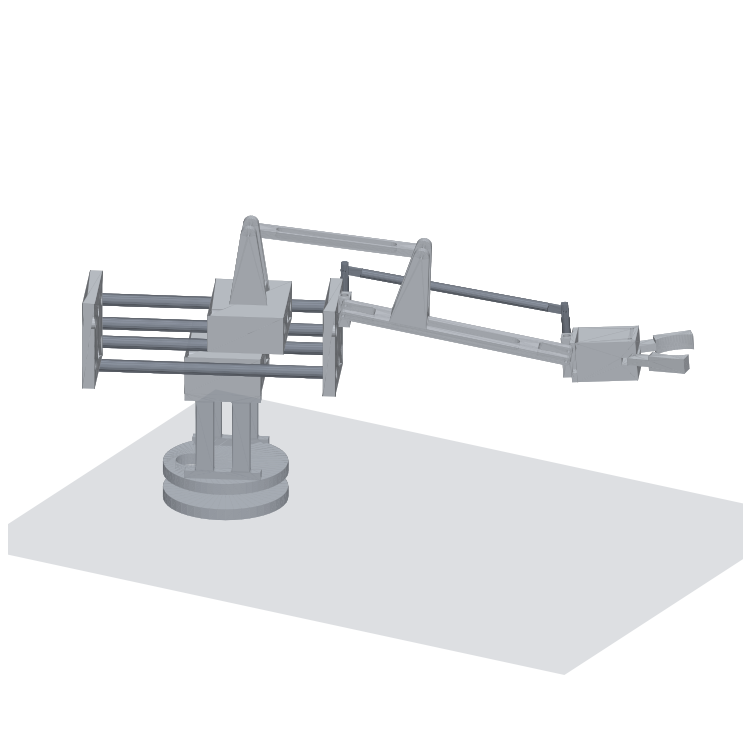
\includegraphics[width=0.48\linewidth]{modelo_3d_isometrica.png}\hfill
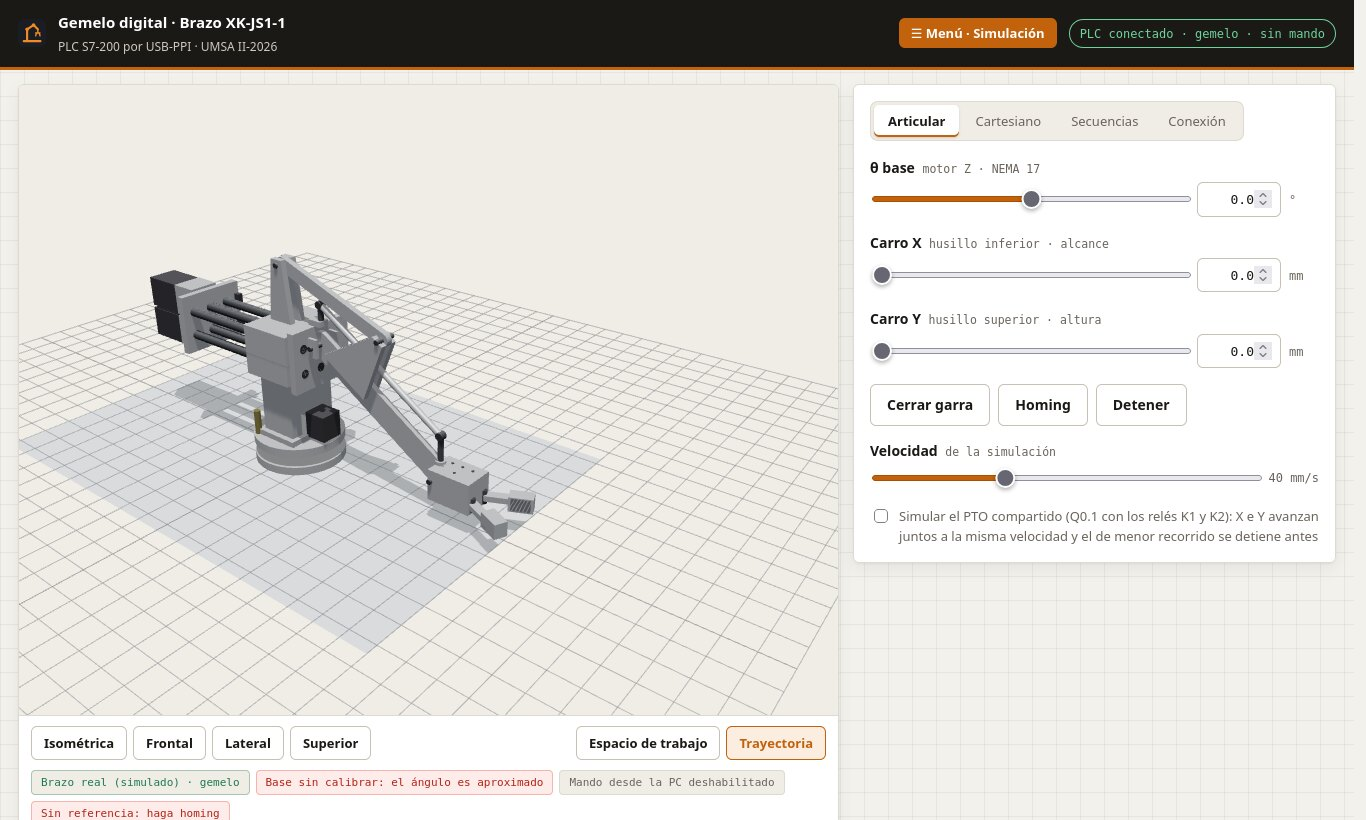
\includegraphics[width=0.48\linewidth, height=5.2cm, keepaspectratio]{gemelo_simulacion.jpg}
\caption{Modelo 3D del brazo (izquierda) y el gemelo en modo simulación dentro de la aplicación (derecha).}
\end{figure}

\subsection{Validación frente a la planta}
\begin{center}\small
\begin{tabularx}{\linewidth}{>{\raggedright}p{6cm} >{\raggedright\arraybackslash}X}
\toprule
\textbf{Prueba} & \textbf{Resultado}\\
\midrule
Geometría del modelo frente a fotos del manual y de la planta & diferencia menor a 5~mm en los pivotes\\
Estimador frente al programa original (\codigo{pruebas\_estimador.py}) & error máximo de 1,35~mm en X e Y\\
Cinemática directa seguida de inversa en toda la grilla & devuelve la misma posición de los carros\\
Posición con el programa \codigo{brazo\_gemelo} cargado & exacta al pulso mientras el motor no pierda pasos\\
\bottomrule
\end{tabularx}
\end{center}
Con un recorrido de 170~mm, el error máximo de 1,35~mm equivale a un ajuste del $1 - 1{,}35/170 = 99{,}2\%$ en posición, por encima del 95\% que pide la guía. \textbf{Advertencia}: este índice compara el estimador con la cuenta de pulsos del PLC, no con una medición independiente de la garra. Falta medir con calibre la posición real en varios puntos (pendiente en el manual técnico) y presentar el índice de ajuste frente a esa medición.

\subsection{Modelo de Simulink e índice de fidelidad}
\paragraph{Simulink.} \codigo{crear\_gemelo\_simulink.m} construye por comandos el modelo \codigo{gemelo\_brazo.slx}: un bloque \emph{From Workspace} con las frecuencias del ensayo escalón (laboratorio 4), el bloque \emph{State-Space} continuo y el \emph{Discrete State-Space} con $G = I$, $H = T_sB$ y $T_s = 25$~ms, y los compara con la posición que informa el PLC. El modelo se genera al ejecutar el script en MATLAB; en la PC de desarrollo no hay MATLAB, así que el \codigo{.slx} no se pudo crear ni probar todavía.

\paragraph{Equivalente en Python.} \codigo{indice\_fidelidad.py --ensayo} hace la misma simulación (continua y discreta ZOH) y calcula el índice de ajuste NRMSE $= 100\,(1 - \lVert y - \hat y\rVert / \lVert y - \bar y\rVert)$, como \codigo{compare} de MATLAB. Con los cuatro ensayos del PLC simulado da entre 99,5 y 99,9~\% (error máximo 0,5~mm, por la resolución de 25~ms). Igual que el 99,2~\% anterior, compara contra la cuenta de pulsos.

\paragraph{Medición independiente (la que pide la firma).} \codigo{indice\_fidelidad.py --calibre medicion\_calibre.csv} compara la posición de la garra que calcula el gemelo con la medida a mano en 11 poses (distancia horizontal $r$ desde el eje de giro y altura $z$ sobre la mesa) e informa el error máximo y el índice $100\,(1 - e_{rms}/268~\text{mm})$. La plantilla ya tiene las poses y la predicción del gemelo; falta medirlas en la planta.

\subsection{Discretización con retención de orden cero}
Del laboratorio 4, cada eje es un integrador: $G(s) = b/s$, con $b = 9{,}17\cdot10^{-5}$~rad/Hz en la base y $b = 0{,}005$~mm/Hz en los carros. Con ZOH:
\[
G(z) = (1 - z^{-1})\,\mathcal{Z}\left\{\frac{b}{s^2}\right\} = (1 - z^{-1})\frac{b\,T_s\,z}{(z-1)^2} = \frac{b\,T_s}{z - 1}.
\]
En espacio de estados, como $A = 0$: $G = e^{AT_s} = I$ y $H = \int_0^{T_s} e^{A\tau}d\tau\,B = T_s B$, es decir
\[
\mathbf{x}(k+1) = \mathbf{x}(k) + T_s\,B(\kappa)\,\mathbf{u}(k),
\]
que es exactamente la ecuación de diferencias que ejecuta el estimador del gemelo: la posición nueva es la anterior más los pulsos del periodo divididos entre los pulsos por unidad.

\subsection{Selección del periodo de muestreo}
La regla $\tau/10 \le T_s \le \tau/4$ supone un polo con constante de tiempo $\tau$. El modelo identificable del brazo no tiene polo (integrador) y la dinámica mecánica no se pudo medir (laboratorio 4), así que \textbf{no se puede aplicar la regla todavía}. Los límites reales del sistema son:
\begin{itemize}
\item \textbf{Actuación}: el programa del PLC envía paquetes de 100 pulsos; a 4~kHz cada paquete dura 25~ms. Un periodo de control menor no puede cambiar la acción a mitad de paquete.
\item \textbf{Comunicación}: cada lectura PPI a 9600~bit/s tarda unos 155~ms (medido). Es el periodo mínimo con el que la PC ve la planta.
\end{itemize}
Por eso se propone $T_s = 25$~ms para un control ejecutado en el PLC (interrupción temporizada, laboratorio 6) y $T_s \approx 155$~ms como periodo de supervisión desde la PC. Cuando se mida $\tau$ con un sensor continuo, se debe verificar que $25~\text{ms} \le \tau/4$.

\section{ETN-1034: propiedades estructurales}
El script \codigo{espacio\_estados\_brazo.py} (y su equivalente \codigo{espacio\_estados\_brazo.m} para MATLAB) calcula las matrices de controlabilidad $M_C = [B\;AB\;A^2B]$ y observabilidad $M_O = [C;\,CA;\,CA^2]$. Resultados (salida completa en \codigo{salida\_espacio\_estados.txt}):

\begin{center}\small
\begin{tabular}{l c l}
\toprule
\textbf{Modo de los relés} & $\operatorname{rango} M_C$ & \textbf{Conclusión}\\
\midrule
K1 cerrado (tren a X) & 2 & no controlable: Y no recibe pulsos\\
K2 cerrado (tren a Y) & 2 & no controlable: X no recibe pulsos\\
K1 y K2 cerrados & 2 & no controlable: X e Y solo con la misma velocidad\\
ninguno & 1 & solo la base\\
conmutando K1 $\leftrightarrow$ K2 & 3 & todos los estados alcanzables por conmutación\\
\midrule
\textbf{Salida} & $\operatorname{rango} M_O$ & \\
\midrule
$C = J(q_0)$ (posición de la garra) & 3 & observable si se midiera la posición\\
sensores reales (finales, inductivo) & -- & salidas binarias: no observable en continuo\\
\bottomrule
\end{tabular}
\end{center}

\paragraph{Interpretación.} Con $A = 0$, $M_C$ se reduce a $[B\;0\;0]$ y su rango es el de $B$. Como X e Y comparten la salida Q0.1, en ningún modo fijo se pueden mover los tres ejes de forma independiente: el sistema \emph{no es apto para realimentación de estados} con la estructura actual. Se vuelve completamente alcanzable conmutando los relés (así trabaja el programa \codigo{brazo\_gemelo}: un tramo común y luego el resto del eje más largo). Para el control avanzado de la fase 3 hace falta: (1) un segundo tren de pulsos o un driver por salida, para que $B$ tenga rango 3, y (2) un sensor continuo de posición, para que la planta sea observable.

\section{ETN-1000: lógica del servidor (PL/pgSQL)}
\subsection{Trigger de seguridad}
La función \codigo{verificar\_limites\_variables()} se ejecuta antes de cada \codigo{INSERT} o \codigo{UPDATE} en la tabla de telemetría (\codigo{muestra}). Si el valor sale del rango de su variable:
\begin{enumerate}
\item registra la alerta \codigo{limite\_variable} en la tabla de alertas (\codigo{evento\_alarma}) con \codigo{clock\_timestamp()}, la hora UTC real con microsegundos;
\item cambia el estado lógico de la planta a falso (\codigo{sistema.en\_operacion = false});
\item desvía el dato: devuelve \codigo{NULL} y la muestra no se guarda.
\end{enumerate}
\begin{lstlisting}[style=sql, caption={Función y trigger (\codigo{database/scripts/brazo\_4gdl.sql}).}]
CREATE FUNCTION verificar_limites_variables() RETURNS trigger AS $$
DECLARE
    r variable%ROWTYPE;
BEGIN
    SELECT * INTO r FROM variable WHERE id = NEW.variable_id;
    IF NEW.valor < r.rango_min OR NEW.valor > r.rango_max THEN
        INSERT INTO evento_alarma (alarma_id, ciclo_id, instante, activa, detalle)
        SELECT a.id, NEW.ciclo_id, clock_timestamp(), true,
               format('%s = %s %s fuera de [%s, %s]', r.tag_isa, NEW.valor, r.unidad, r.rango_min, r.rango_max)
        FROM alarma a WHERE a.codigo = 'limite_variable';
        UPDATE sistema SET en_operacion = false
        WHERE id = (SELECT sistema_id FROM ciclo_operacion WHERE id = NEW.ciclo_id);
        RAISE WARNING 'muestra descartada: % = % % fuera de [%, %]',
            r.tag_isa, NEW.valor, r.unidad, r.rango_min, r.rango_max;
        RETURN NULL;
    END IF;
    RETURN NEW;
END;
$$ LANGUAGE plpgsql;
CREATE TRIGGER muestra_en_rango BEFORE INSERT OR UPDATE ON muestra
    FOR EACH ROW EXECUTE FUNCTION verificar_limites_variables();
\end{lstlisting}

\paragraph{Por qué \codigo{RETURN NULL}.} Si el trigger lanzara una excepción, PostgreSQL desharía toda la transacción, \emph{incluida la alerta}: la falla quedaría sin registro. Con \codigo{RETURN NULL} se omite solo la fila de la muestra y la alerta y el cambio de estado se conservan. Es un comportamiento determinista: el mismo dato inválido produce siempre la misma alerta.

\paragraph{Umbrales.} Los límites son los recorridos físicos de la planta, guardados en \codigo{variable}: base de $-263°$ a $263°$, carros X e Y de 0 a 170~mm, trenes de 0 a 20\,000~Hz (máximo del PTO de la CPU 224). Una muestra fuera de ese rango indica un error del estimador, una pérdida de referencia o un dato corrupto: es la «colisión angular del brazo» que menciona la guía.

\subsection{Pruebas de inyección}
El script \codigo{database/scripts/prueba\_reglas.sql} inyecta valores erróneos dentro de una transacción que se deshace al final:
\begin{center}\small
\begin{tabularx}{\linewidth}{c >{\raggedright}X >{\raggedright\arraybackslash}p{5.6cm}}
\toprule
\textbf{Nº} & \textbf{Inyección} & \textbf{Resultado esperado}\\
\midrule
1 & ZI-102 = 85~mm & la muestra se guarda\\
2 & ZI-102 = 250~mm & descartada, alerta registrada, planta fuera de operación\\
3 & valor nulo & rechazada por NOT NULL\\
4 & ciclo en modo «turbo» & rechazado por CHECK\\
5 & variable inexistente (999) & rechazada por la clave foránea\\
6 & tag ZS-101 repetido & rechazado por UNIQUE\\
7 & borrar ZI-102 con historial & impedido por ON DELETE RESTRICT\\
\bottomrule
\end{tabularx}
\end{center}
\paragraph{Resultado de la ejecución} (PostgreSQL 16.2, 12/11/2026, PC de desarrollo; registro completo en \codigo{database/scripts/registro\_ejecucion.txt}):
\begin{lstlisting}[basicstyle=\ttfamily\scriptsize]
 prueba 1 correcta: muestra en rango aceptada
WARNING:  muestra descartada: ZI-102 = 250 mm fuera de [0, 170]
NOTICE:  prueba 2 correcta: 250 mm descartado, alerta registrada y planta fuera de operación
NOTICE:  prueba 3 correcta: null value in column "valor" of relation "muestra" violates not-null constraint
NOTICE:  prueba 4 correcta: new row for relation "ciclo_operacion" violates check constraint "ciclo_operacion_modo_check"
NOTICE:  prueba 5 correcta: insert or update on table "muestra" violates foreign key constraint "muestra_variable_id_fkey"
NOTICE:  prueba 6 correcta: duplicate key value violates unique constraint "punto_io_tag_isa_key"
NOTICE:  prueba 7 correcta: update or delete on table "variable" violates foreign key constraint "muestra_variable_id_fkey"
\end{lstlisting}
Con 18\,000 muestras sintéticas ya cargadas se repitió la inyección de un valor extremo (base a 400°): el \codigo{INSERT} devolvió \codigo{INSERT 0 0} (dato desviado), quedó la alerta «ZI-101 = 400 deg fuera de [-263, 263]» y \codigo{sistema.en\_operacion} pasó a falso. La primera corrida detectó un error en el propio script de pruebas (la prueba 5 fallaba por el ciclo y no por la variable, porque una inserción rechazada consume la secuencia); se corrigió y se repitió.

\section{Entregables (Definition of Done)}
\begin{dod}
Archivos de simulación (.slx / .m) con el gemelo y el rango de matrices & \parcial & gemelo en la app, \codigo{espacio\_estados\_brazo.m}/\codigo{.py}, \codigo{crear\_gemelo\_simulink.m} (genera el \codigo{.slx}; sin ejecutar por falta de MATLAB) e \codigo{indice\_fidelidad.py}\\
Índice de fidelidad frente a la planta (más de 95~\%) & \parcial & procedimiento y plantilla \codigo{medicion\_calibre.csv} listos; faltan las mediciones con calibre\\
Script SQL de lógica de servidor (PL/pgSQL) & \cumple & \codigo{database/scripts/brazo\_4gdl.sql} y \codigo{prueba\_reglas.sql}, ejecutados en PostgreSQL 16.2 (\codigo{registro\_ejecucion.txt})\\
Informe de cierre de fase 2 & \cumple & este informe, con el del laboratorio 4\\
Firma del escudo de seguridad del docente & \falta & pendiente de la revisión del docente\\
\end{dod}

\section{Conclusiones}
\begin{enumerate}
\item El gemelo digital reproduce la geometría con menos de 5~mm de error y el estimador sigue al PLC con un error máximo de 1,35~mm; falta contrastarlo con una medición independiente.
\item La discretización con ZOH de un integrador da $\mathbf{x}(k+1) = \mathbf{x}(k) + T_sB\mathbf{u}(k)$, la misma ecuación que ya ejecuta el estimador.
\item El análisis estructural muestra el límite de la planta: con un solo tren de pulsos para X e Y y sin sensores continuos, el sistema no es controlable en ningún modo fijo ni observable. El control por realimentación de estados de la fase 3 requiere cambios de hardware.
\item El trigger de seguridad cumple la lógica que pide la guía (desviar, alertar y detener) y se comprobó en PostgreSQL 16.2 con inyecciones de datos erróneos.
\end{enumerate}

\end{document}
